\documentclass[conference]{IEEEtran}
\IEEEoverridecommandlockouts
% The preceding line is only needed to identify funding in the first footnote. If that is unneeded, please comment it out.
\usepackage{cite}
\usepackage{amsmath,amssymb,amsfonts}
\usepackage{graphicx}
\usepackage{textcomp}
\usepackage{xcolor}
\usepackage{algorithm} 
\usepackage{algpseudocode} 
\def\BibTeX{{\rm B\kern-.05em{\sc i\kern-.025em b}\kern-.08em
    T\kern-.1667em\lower.7ex\hbox{E}\kern-.125emX}}
\begin{document}

\title{Simulated Annealing Approach to ICCAD Contest Problem A: Reinforcement Logic Optimization for a General Cost Function\\}


\author{\IEEEauthorblockN{1\textsuperscript{st} Oniontow Ren-Xuan Wang}
\IEEEauthorblockA{\textit{Department of Electrical Engineering} \\
\textit{of National Taiwan University}\\
Taipei, Taiwan. \\
}
\and
\IEEEauthorblockN{2\textsuperscript{nd} Boyuan Cheng}
\IEEEauthorblockA{\textit{Department of Electrical Engineering} \\
\textit{of National Taiwan University}\\
Taipei, Taiwan. \\
}
\and
\IEEEauthorblockN{3\textsuperscript{rd} Stanley Huang}
\IEEEauthorblockA{\textit{Department of Electrical Engineering} \\
\textit{of National Taiwan University}\\
Taipei, Taiwan. \\
}
}

\maketitle

\begin{abstract}
This is the final report of Introduction to Electronic Design Automation, using simulated annealing technique to resolve problem A of ICCAD contest 2024.
The overall process contains two parts: logic synthesis and technology mapping. We use Berkeley ABC tool to do logic synthesis, and applied our process to design1.v in the benchmark of the ICCAD contest. We found that to some cost estimators, logic synthesis parts can have great performance, but technology mapping does not affect much. While for other cost estimators, logic synthesis process does not have significant impact, while technology mapping performs well.
\end{abstract}

\begin{IEEEkeywords}
simulated annealing, logic synthesis, handsome oniontow
\end{IEEEkeywords}

\section{Problem Description}

We are given a specified netlist in verilog format, a cell library in json-liked format that contains parameters of some primitive gates, and a black-box cost estimator.

\subsection{Netlist}

The input netlist is a flattened netlist in Verilog format without hierarchy (one top module only).\\
The netlist is composed of:\\
1. primitive gates (and, or, nand, nor, not, buf, xor, xnor)\\
2. wires\\
3. constant values (1’b1, 1’b0)\\
All primitive gates are assumed to have only 2 inputs and 1 output
except for buffer and not gates, which have only 1 input and 1 output.
All primary inputs and primary outputs are scalars (i.e., one-bit signals)\\

\subsection{Cell library}

For each primitive gate, at least one cell exists in the cell library.\\
The first section is information (a json object) with three properties. The first property is cell\_num, which states the number of cells in the cell library. The second property is attribute\_num, which states the number of attributes in each cell. The third property is attributes, in which there are
attribute\_num strings in the json-array denoting the property names of the
attributes of each cell.
The second section is cells, which is a json array. There are exactly
\#cell\_num cells described in this section. For each cell, exactly
\#attribute\_num properties are specified. Fig. 1 shows an example of part of the cell library.
\begin{figure}
    \centering
    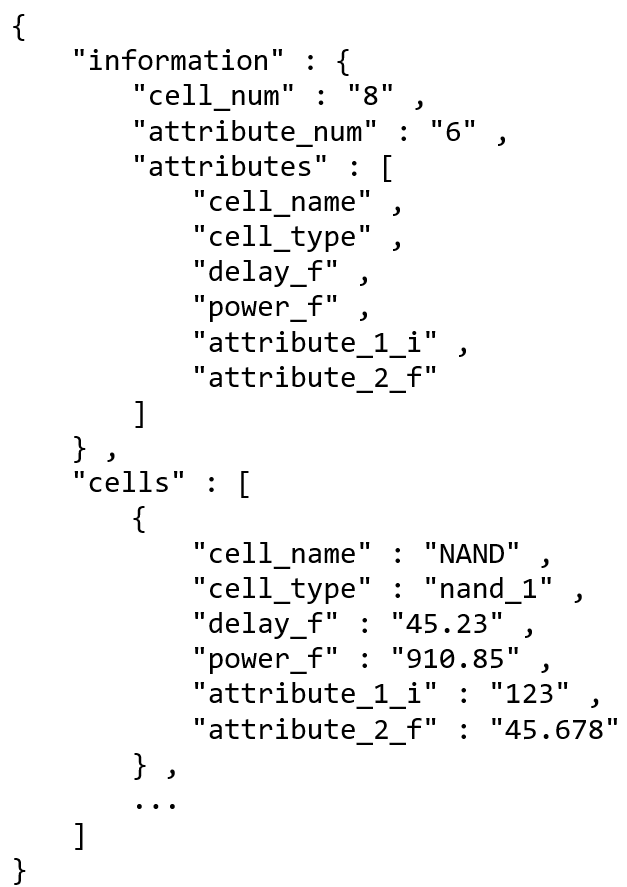
\includegraphics[width=0.6\linewidth]{example of cell library.png}
    \caption{Example of cell library}
    \label{fig:enter-label}
\end{figure}

\subsection{Cost function estimator}
The cost function estimator is an executable file, which takes 2 input files and generates 1 output file. The input files are a cell library and a netlist. All the gates in the netlist should be specified by the cell library. The output file contains a floating number which denotes the cost of the netlist.

\section{Simulated Annealing Strategy}

When we get a netlist, we first want to logic synthesis and reduction to the netlist due to a naive thought that less gates leads to less cost (in area, power, or other properties). 

After doing proper logic synthesis, We will get a gate-level verilog file. Then we can map those gates in the verilog file to the gates specified in the cell library. 

To furthur improve the performance, We can first find the gates specified in the cell library that are more suitable for the given cost estimator. 

Those gates is used as the fast technology mapping of the logic gates in logic reduction part, and initial condition of the technology mapping part.

For the procedures above, we use simulated annealing method to find a decent cost. Fig. 2 shows the flow chart of our process.

\begin{figure}
    \centering
    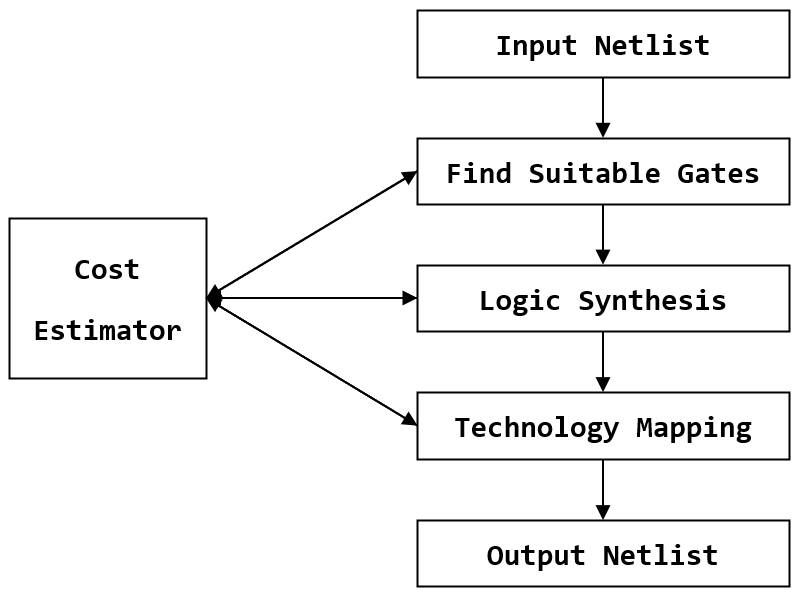
\includegraphics[width=1\linewidth]{flow chart.png}
    \caption{Flow Chart of Overall Process}
    \label{fig:enter-label}
\end{figure}

\subsection{Find Suitable gates}

For the beginning part, We create a fake netlist that contains only one of the primitive gates. Then we assign the gate all kinds of types to the gates, greedily pick the best assignment of the netlist. After doing this process to all primitive gates, we can get a dictionary that contains best types of all primitive gates. Here shows the pseudo code of finding the most suitable gates.

\begin{algorithm}
\begin{algorithmic}[1]
    \caption{Find-Suitable-Gates}\label{euclid}
    \State BestType = $\emptyset $
    \For {gate $\in$ gates}
    \State CurrentBest $\gets \infty$ 
        \For {type $\in $ types}
            \If {CostEstimator(gate[type]) $<$ CurrentBest}
                \State CurrentBest $\gets$ type
            \EndIf
        \EndFor
        \State BestType $\gets $ BestType $\cup $ \{gate:CurrentBest\}
    \EndFor
    \State \Return BestType
\end{algorithmic}
\end{algorithm}

\subsection{Logic Synthesis}

For the logic synthesis part, We conduct operations on the netlist with the help of Berkeley ABC. We first convert the netlist to And-Inverter-Graph(AIG), then do simulated annealing on the AIG. For simulated annealing, we define the process with the following conditions.\\

\subsubsection{Action Space}

Action space of the logic synthesis process is a set of some ABC commands such as $resyn$, $fx$, $compress$, $dc2$ $\dots$ .

\subsubsection{Neighborhood Structure}

The neighborhood of each AIG is all AIGs produces by conducting one command in the action space.

\subsubsection{Cost Function}

Cost function is defined by the given cost estimator.\\

In every iteration of the simulated annealing loop, we randomly jump to a random neighborhood state, then we map the current AIG to netlist output in verilog format using the dictionary of most suitable gates if given. If not, we simply assign all gates to type 1 for time-saving consideration. After doing so, we can get the cost from cost estimator. Here we show the pseudo code of our simulated annealing process.

\begin{algorithm}
\begin{algorithmic}[1]
    \caption{Simulated-Annealing-of-Logic-Synthesis}\label{euclid}
    \State ActionSpace $ \gets \{ $ABC Commands$ \}$
    \State CurrentState $\gets$ netlist
    \State CurrentCost $\gets$ Cost(CurrnetState, SuitableGates)
    \State T $\gets$ $T_0$
    \While {T $>$ $T_{min}$}
        \State Neighbor $\gets \emptyset$
        \For{action $\in$ ActionSpace}
            \State Neighbor $\gets$ Neighbor $\cup$ CurrentState.action
        \EndFor
        \State NextState $\gets$ Random(Neighbor)
        \State NextCost $\gets$ Cost(NextState, SuitableGates)
        \If{NextCost $<$ CurrentCost}
            \State CurrnetState $\gets$ NextCost
            \State CurrentCost $\gets$ NextCost
        \ElsIf{Random(0,1) $>\ e^{-\frac{NextCost - CurrentCost}{T}}$}
            \State CurrnetState $\gets$ NextCost
            \State CurrentCost $\gets$ NextCost
        \EndIf
    \EndWhile
\end{algorithmic}
\end{algorithm}

\subsection{Technology Mapping}

In the technology mapping part, we map the synthesized netlist to primitive gates specified in the library. If we have a dictionary of most suitable gates as input, then we assign all gates to the types given in the dictionary as initial condition. If not, then we randomly assign a type to each gate. For simulated annealing, we define the process with the following conditions.\\


\subsubsection{Action Space}

Action space of the technology mapping part is modifying the type of some gates in the synthesized netlist. The modified gates will get a new randomly assigned type.

\subsubsection{Neighborhood Structure}

The neighborhood of each netlist is all netlists that exactly one gate in the netlist has different type to the original netlist.

\subsubsection{Cost Function}

Cost function is defined by the given cost estimator.\\

In every iteration of the simulated annealing loop, we consequently jumps to a new neighbor state for several times that is roughly proportional to the current temperature and the length of the netlist. That is, we jump to furthur states in the beginning, and we jump to closer states when the temperature is low. If not doing this adjustment, the time required for the simulated annealing process will greatly depend on the length of the netlist, and the performance will worsen significantly if we use same parameters as those we used for small netlists. Therefore, To keep the process and the code have more compatibility and can simplify the parameter choosing problem for us. To be precise, we use the following pseudo code to determine how far should we jump to.
\begin{algorithm}
\begin{algorithmic}[1]
    \caption{Jumping-Steps}\label{euclid}
    \State Step $\gets 100\ \times $ netlist.length $\times\ \frac{T}{T_{max}}$ 
    \If{Step $>$ netlist.length}
        \State Step $\gets$ netlist.length
    \ElsIf{Step $<$ 1}
        \State Step $\gets \ 1$
    \EndIf
    \State \Return Step
\end{algorithmic}
\end{algorithm}

Then we can get a modified simulated annealing pseudocode.

\begin{algorithm}
\begin{algorithmic}[1]
    \caption{Simulated-Annealing-of-Technology-Mapping}\label{euclid}
    \State CurrentState $\gets$ netlist
    \State CurrentCost $\gets$ Cost(CurrnetState, SuitableGates)
    \State T $\gets$ $T_0$
    \While {T $>$ $T_{min}$}
        \State Step $\gets$ Jumping-Steps(T, netlist.length)
        \For{step $\in$ Step}
            \State CurrentState $\gets$ NextState
        \EndFor
        \State NextCost $\gets$ Cost(NextState, cell-lib)
        \If{NextCost $<$ CurrentCost}
            \State CurrnetState $\gets$ NextCost
            \State CurrentCost $\gets$ NextCost
        \ElsIf{Random(0,1) $>\ e^{-\frac{NextCost - CurrentCost}{T}}$}
            \State CurrnetState $\gets$ NextCost
            \State CurrentCost $\gets$ NextCost
        \EndIf
    \EndWhile
\end{algorithmic}
\end{algorithm}

\section{Results}
We are going to summarize our different methods to reduce the cost and show the optimization results of those methods in Table I.\\

\subsection{Baseline}
We define the baseline as the cost of the original netlist with all gate assigned type I. Thus, we define the performance ratio of a netlist be the ratio of the new cost and the baseline. \\
$\text{PRN} = \frac{\text{cost of the netlist}}{\text{cost of original netlist (assigned type I)}}$ \\
The lower the ratio is, the performance is better. Noting that if the baseline is already zero, it is good enough. Thus, we define PRN be zero if the cost of new netlist is zero.\\

\subsection{Suitable gates (SG)}
Also, as mentioned before, we find suitable gates in the beginning of the process by letting cost estimator give the cost of only one gate. We apply this assignment on the whole circuit and in some cases there is significant improvement. \\

\subsection{Suitable gates + Technology mapping annealing (SG+TSA)}
We do Simulated-Annealing-of-Technology-Mapping start from assigning the suitable gates first. This performance indicate the efficiency of the second simulated annealing.
\\

\subsection{Suitable gates + Logic synthesis simulating annealing (SG+LSA)}
We do Simulated-Annealing-of-Logic-Synthesis to get the combinational circuit and assign suitable gates to get cost. This performance indicate the efficiency of the first simulated annealing.
\\

\subsection{The whole process (SG+LSA+TSA)}
This given netlist undergo the process shown in Fig.2. In fact, this is the result of the combination of the previous one and TSA.
\\
\\
We run our algorithm on design1.v in the benchmark provided by the ICCAD contest, Table I shows our result:

\begin{table}[htbp]
\caption{Performance of design1.v}
\begin{center}
\begin{tabular}{|c|c|c|c|c|c|c|c|c|}
\hline
\textbf{Table}&\multicolumn{8}{|c|}{\textbf{Cost estimator type}} \\
\cline{2-9} 
\textbf{Head} & 
\textbf{\textit{1}}& 
\textbf{\textit{2}}&
\textbf{\textit{3}}&
\textbf{\textit{4}}&
\textbf{\textit{5}}&
\textbf{\textit{6}}&
\textbf{\textit{7}}&
\textbf{\textit{8}} \\
\hline
Baseline&7.402&28.384&1.671&6.645&1.037&0.0&2.002E+7&2.592\\
\hline

SG&3.271&17.678&1.444&3.933&1.007 &0.0 &2.002E+7&2.543\\
\cline{2-9}
PRN&0.442&0.623&0.864&0.592&0.971&0&1.000&0.981\\
\hline

SG+TSA&3.271&12.495&1.444&3.933&1.007 &0.0 &2.002E+7&2.543\\
\cline{2-9}
PRN&0.442&0.440&0.864&0.592&0.971&0&1.000&0.981\\
\hline

SG+LSA&3.290 &28.384&1.671&3.948&1.008&0.0&2.002E+7&2.049\\
\cline{2-9}
PRN&0.444&1&1&0.594&0.972&0&1.000&0.790\\
\hline

Whole&3.290 &13.180&1.543&3.948&1.008&0.0&2.002E+7&2.049\\
\cline{2-9}
PRN&0.444&0.464&0.923&0.594&0.972&0&1.000&0.790\\
\hline

%\multicolumn{4}{l}{$^{\mathrm{a}}$Sample of a Table footnote.}
\end{tabular}
\label{tab1}
\end{center}
\end{table}

Also, from Table I, we observe that the whole process leads to the most cost reduction. Therefore, in our remaining data, we only apply the whole process to design 2-6 to obtain data to analyze our annealing procedure. The data is shown in Table II.

\begin{table*}[htbp]
\caption{Performance of design2-6.v}
\begin{center}
\begin{tabular}{|c|c|c|c|c|c|c|c|c|c|}
\hline
&\textbf{}&\multicolumn{8}{|c|}{\textbf{Cost estimator type}} \\
\cline{3-10}
\textbf{} & 
\textbf{} & 
\textbf{\textit{1}}& 
\textbf{\textit{2}}&
\textbf{\textit{3}}&
\textbf{\textit{4}}&
\textbf{\textit{5}}&
\textbf{\textit{6}}&
\textbf{\textit{7}}&
\textbf{\textit{8}} \\
\cline{1-10}
  & baseline & 153.45536 & 44.84497 & 1.455316 & 48.51754 & 1.758219 & 45       & 20456129 & 5.789047 \\
\cline{2-10}
2 & whole    & 69.302068 & 3.334768 & 1.321251 & 29.42091 & 1.156148 & 44       & 20456058 & 4.743037 \\
\cline{2-10}
  & PRN      & 0.4516106 & 0.074362 & 0.907879 & 0.606397 & 0.657568 & 0.977778 & 0.999997 & 0.819312 \\
\hline
  & baseline & 176.76066 & 9.867051 & 1.233892 & 52.53959 & 1.900393 & 27       & 20590149 & 6.065078 \\
\cline{2-10}
3 & whole    & 79.920518 & 1        & 1.030533 & 31.00437 & 1.185331 & 24       & 20590067 & 4.69313  \\
\cline{2-10}
  & PRN      & 0.4521397 & 0.101347 & 0.835189 & 0.590114 & 0.623729 & 0.888889 & 0.999996 & 0.773795 \\
\hline
  & baseline & 1279.3728 & 5058.617 & 1.427662 & 196.3543 & 5.585199 & 0        & 23439129 & 11.65184 \\
\cline{2-10}  
4 & whole    & 553.09128 & 5058.617 & 1.427662 & 128.1597 & 1.859432 & 0        & 23438488 & 9.271787 \\
\cline{2-10}
  & PRN      & 0.4323144 & 1        & 1        & 0.652696 & 0.332921 & 0        & 0.999973 & 0.795736 \\
\hline
  & baseline & 1419.1928 & 717.1672 & 1.764288 & 214.4833 & 8.073558 & 384      & 22421199 & 13.50772 \\
\cline{2-10}  
5 & whole    & 641.48838 & 436.7219 & 1.75488  & 131.0182 & 2.458844 & 384      & 22420541 & 9.890754 \\
\cline{2-10}
  & PRN      & 0.4520093 & 0.608954 & 0.994668 & 0.610855 & 0.304555 & 1        & 0.999971 & 0.73223  \\
\hline
  & baseline & 3007.0463 & 479.0044 & 1.543557 & 347.5543 & 18.05939 & 1143     & 24922487 & 17.70281 \\
\cline{2-10}
6 & whole    & 1359.0843 & 434.7397 & 1.517821 & 212.4604 & 4.497268 & 1143     & 24921123 & 12.55958 \\
\cline{2-10}
  & PRN      & 0.4519665 & 0.90759  & 0.983327 & 0.611301 & 0.249027 & 1        & 0.999945 & 0.709468 \\
\hline


%\multicolumn{4}{l}{$^{\mathrm{a}}$Sample of a Table footnote.}
\end{tabular}
\label{tab1}
\end{center}
\end{table*}

\section{Discussion}
We observe some phenomenon and are going to discuss in the following.\\
\subsubsection{}
We found that both simulated annealing (Logic synthesis and technological mapping) are important. For cost estimator 2, technological mapping takes crucial part. For others, logical synthesis has great effect.
\\
\subsubsection{}
We see that the result of logic synthesis may impact the effect of technological mapping simulated annealing, as the structure of the circuit has been changed. Thus, going through the whole process may lead to a good expected result but may not be the best. 
\\
\subsubsection{}
For cost estimator 7, every method listed above cannot significantly make the costs lower. We think this phenomenon occurs due to the bias of the model. Such as in our observation of the Technology mapping Simulated Annealing (TSA) part, the buffers in the netlist-to-be-optimized will be wiped out, and there is no way to retrieve the information of the buffers or add new buffers. These kinds of biases exists in our annealing process, but their effect is not in our consideration.
\\
\subsubsection{}
Fig.3 shows the relation between the final cost we get and the initial temperature for TSA (Technology mapping Simulated Annealing). We can see that when the initial temperature is set about at 0.1 degree, the performance is very good. If the temperature increases, the standard deviation may decrease and the average cost is slightly decreased. We utilize initial temperature 1000 to be the starting point for the experiment ,for we regard it as a balanced point between time cost and performance.

\begin{figure}
    \centering
    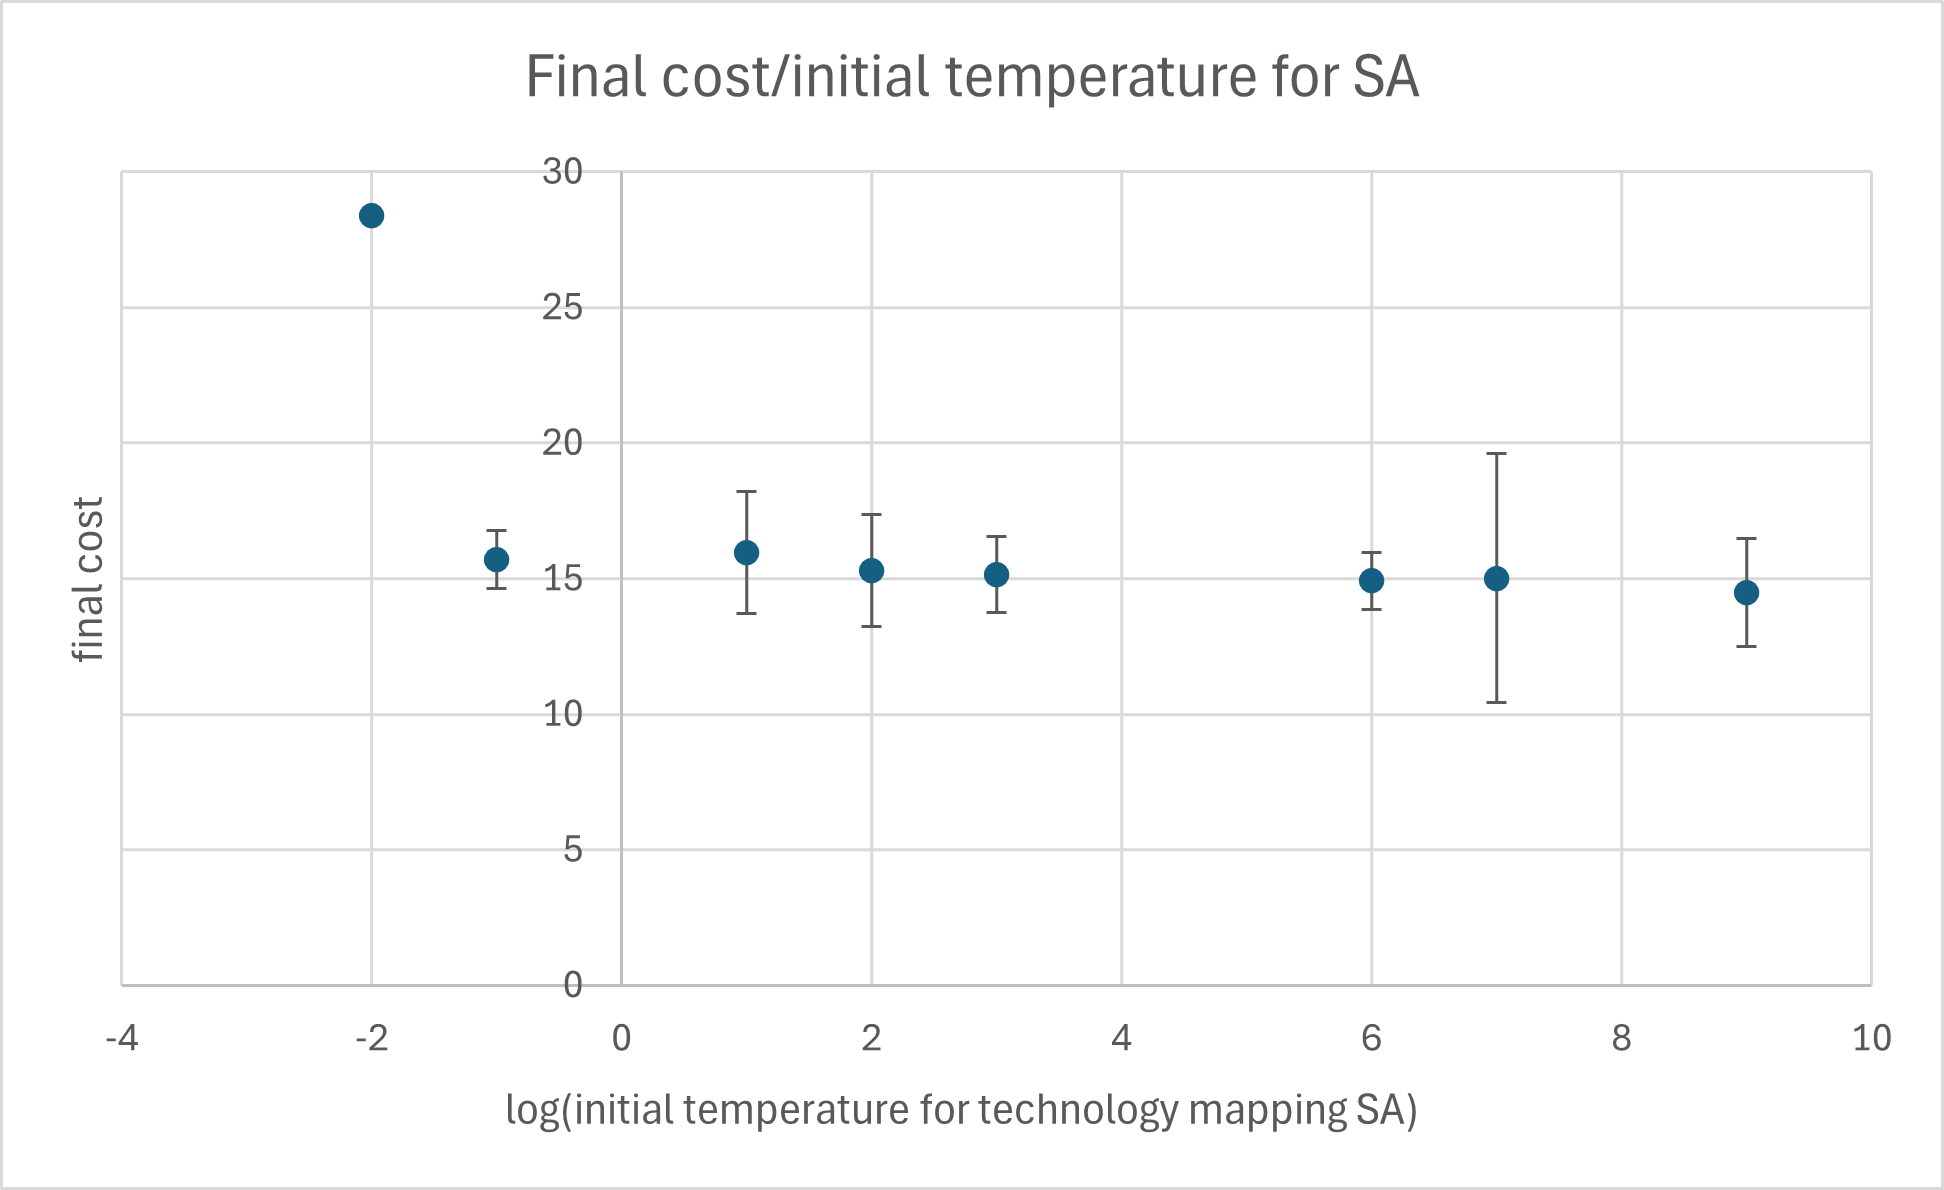
\includegraphics[width=0.99\linewidth]{cost.png}
    \caption{Result with different initial temperature for SA}
    \label{fig:enter-label}
\end{figure}

\section{Job division}
B11901020 Boyuan Cheng: read data from verilog file, find suitable gates, SA analysis according to temperature, performance recording, report.\\
B11901027 Renxuan Wang: Programming part of LSA and TSA, adjustment of simulated annealing parameters, functions of outputting verilog-format results, report.
\\
\begin{thebibliography}{00}
\bibitem{b1} ABC: System for Sequential Logic Synthesis and Formal Verification. https://github.com/berkeley-abc/abc
\bibitem{b1} ICCAD Cad Contest: Reinforcement Logic Optimization for a General Cost Function. https://drive.google.com/file/d/1AfxpS7q7OEg5QP06wgk1rrVqZroT7Ypi/view
\end{thebibliography}
\end{document}
